% This file contains the sections, paragraphs, and figures I deleted
% after a first-pass on 2023-08-24.

% From synthetic oscillations report
In the time series analysis literature, there is a wealth of analysis methods that aim to find parameters pertaining to the periodicity of noisy time series and that aim to characterise the relationship between two signals.
This is relevant for biological time series, especially because they are noisy due to both intrinsic and extrinsic noise sources, and because researchers often record multiple time series from the same system to study the relationship between such time series.
One example is the yeast metabolic cycle, which is known to be a metabolic oscillator that is coupled with the cell division cycle oscillator.
In this case, the two time series from this system consist of the level of metabolites to represent the metabolic oscillator and the activity of a component of the cell division cycle to represent the cell division cycle.

The first step of any data science pipeline is cleaning data.% , and of course there is the adage: 80\% of data science is cleaning data [CITATION NEEDED].
Cleaning data is important because of `garbage in, garbage out': regardless of how cutting-edge the analysis methods are, if the input data is flawed, the data analyst cannot obtain good insights from the data.
However, this step involves judgement calls: the analyst needs to decide on criteria to separate useful data from useless data.
These criteria may be based on existing standards of practice or, for systems biology, knowledge of either the underlying biological processes or of the mathematical constraints.
Often, these criteria can be arbitrary because there is an absence of existing standards of practice for the specific situation --- in this case, any decision is going to be a trade-off and needs justification.

\begin{figure}
  \centering
  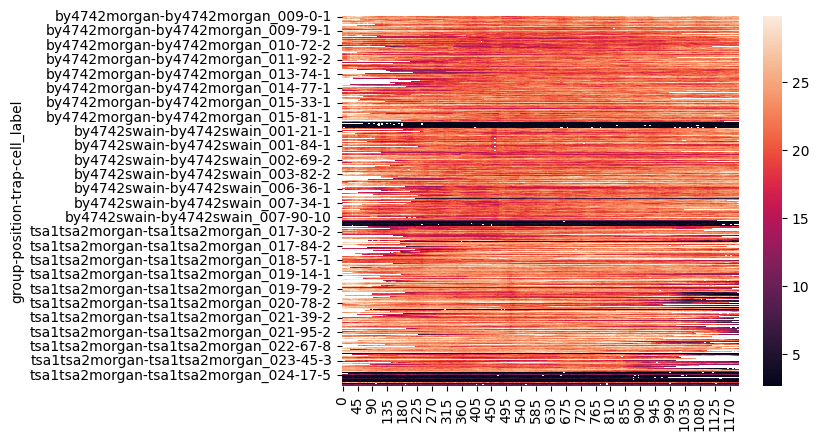
\includegraphics[width=0.9\textwidth]{example_dataframe_heatmap}
  \caption[
    Heatmap of example dataframe
  ]{
    Heatmap of example dataframe shown in figure~\ref{fig:analysis-example-dataframe}.
    Each row represents a cell, each column represents a time point, and the colour of the pixel (colour bar, right) represents the fluorescence intensity.
    Some cells are not present for the whole time course of the experiment, and errors in the segmentation pipeline produce missing time points seen as white pixels in the heatmap.
  }
  \label{fig:analysis-example-heatmap}
\end{figure}

For example, in climate science, if there is a time series of atmospheric \ce{CO2} over a period of decades, we would like to filter out the annual (seasonal) cycles and look at the long-term changes over time.

Next, missing time points can pose a problem, especially when many analysis methods assume evenly-spaced time series. %[WHICH?]
The Lomb-Scargle periodogram \parencite{lombLeastsquaresFrequencyAnalysis1976} is a method developed for problems like this.
Specifically, it was developed for astronomical data that often has missing time points, corresponding to cloud cover, for example.
In my analysis, cases of missing time points are few and could be resolved by linear interpolation, so I will not discuss in detail methods to handle missing time points.


The spectra (figure~\ref{fig:analysis-svc-fft}) suggest that oscillatory cells exhibit a peak, corresponding to features 6--7, that is absent in non-oscillatory cells.
The peak corresponds to a period of 70--80 minutes.
This peak may explain the good precision \& recall scores.

\begin{figure}
  \centering
  \begin{subfigure}[htpb]{0.7\textwidth}
   \centering
   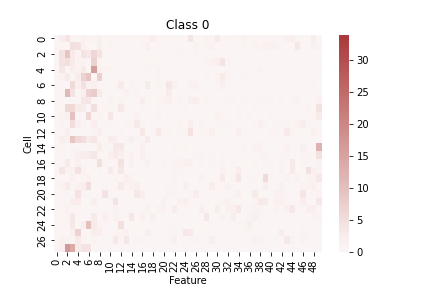
\includegraphics[width=\textwidth]{fft_testing_featurevector_0}
   \caption{
   }
   \label{fig:analysis-svc-fft-0}
  \end{subfigure}

  \begin{subfigure}[htpb]{0.7\textwidth}
   \centering
   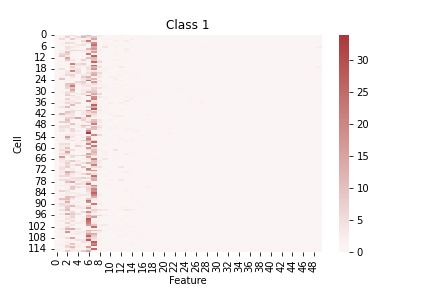
\includegraphics[width=\textwidth]{fft_testing_featurevector_1}
   \caption{
   }
   \label{fig:analysis-svc-fft-1}
  \end{subfigure}
  \caption[
    Fourier spectra of cells in testing set
  ]{
    Fourier spectra of cells in testing set classified as non-oscillatory (class 0,~\ref{fig:analysis-svc-fft-0}) and oscillatory (class 1,~\ref{fig:analysis-svc-fft-1}) by an SVC.
    Rows represent each cell, each used as an observation for the model.
    Columns represent each discrete frequency, used as a features for the model.
    Shades of red represent the power at each discrete frequency, used as feature values.
  }
  \label{fig:analysis-svc-fft}
\end{figure}


\textcite{zielinskiStrengthsLimitationsPeriod2014} discuss several methods, including: FFT NLLS (non-linear least squares, described by \textcite{straumeLeastSquaresAnalysisFluorescence2002}), MFourFit \parencite{edwardsQuantitativeAnalysisRegulatory2010}, MESA (maximum entropy spectral analysis, described by \textcite{burgRelationshipMaximumEntropy1972}), and the Lomb-Scargle periodogram \parencite{lombLeastsquaresFrequencyAnalysis1976}.

% I probably need to try out at least the first two
\begin{description}
    \item [FFT NLLS] \hfill \\

        \begin{itemize}
          \item Is based on the assumption that the time series is best modelled by a sum of cosine functions, each with its own period, amplitude, and phase.
                In general, five cosines are sufficient for most biological data.
          \item First fits the data with one cosine and adjust the period, amplitude, and noise parameters using the non-linear least squares fitting algorithm.
                The Fast Fourier Transform (FFT) can be performed to find a good set of initial parameters.
                Subsequent cosines are added and their parameters found using the same process until new cosines do not significantly improve the fit.
          \item The confidence levels of the parameters are found by varying the parameter values until the resulting fit significantly differs from the best-fit model.
                These can be expressed in terms relative to the original best-fit parameter values.
          \item The period of the time series is reported as the period of the cosine that gives the best fit and is within the expected range of periods.
                Skewness does not affect period.
        \end{itemize}

    \item [MFourFit] \hfill \\

        \begin{itemize}
          \item Is based on fitting one principal cosine and up to four additional cosines, as a way to reduce model complexity.
                Each cosine has a period, amplitude, and phase parameter, but the phase parameters of each additional cosine is define as a fraction $\frac{1}{2}, \frac{1}{3}, \ldots \frac{1}{5}$ of the principal cosine.  These harmonics describe the shape of oscillations.
          \item This algorithm does not directly estimate a period, but varies its estimating of the period within a range of user-defined values.
                The algorithm evaluates the fit by computing the sum of squared differences between the model and the data, and the model is chosen based on the best fit.
          \item This algorithm always returns a period even if the time series is not oscillatory.
                It also assumes knowledge of the shape, and skewness does not affect period.
        \end{itemize}

    \item [MESA] \hfill \\

        \begin{itemize}
          \item Unlike previous curve-fitting methods, MESA fits an autoregressive model to the data then gets period from it.
                The autoregressive model assumes that each data point can be expressed as the linear combination of a defined number of time points before it (the order), plus noise.
                This fitted model leads to an analytical expression of the frequency spectrum, and the period can be found from this expression.
          \item Choosing the best order can be a form of model selection.
          \item Does not assume a shape of the waveform, and is more precise that Fourier-based methods, but lacks a confidence measure.
                Empirically does well and fast.
                It is based on a very different principle than MFourFit, so if both methods agree on the value of the period, then we can be confident that we have the correct period.
        \end{itemize}

    \item [Lomb-Scargle periodogram] \hfill \\

        \begin{itemize}
            \item Fits one sinusoid, assumes a period.
            \item Choose one that gives least error.
            \item Can be used with data with time points that are not evenly spaced
        \end{itemize}

\end{description}

For further detail, I discussed MESA in section~\ref{subsec:analysis-classification-ar} and the Lomb-Scargle periodogram in section~\ref{subsec:analysis-classification-spectral}.

% First-order DEs redundant?
or as a system of first-order differential equations:

\begin{equation}
  \begin{aligned}
    \ndif{y}{t} &= v \\
    \ndif{v}{t} &= -\omega^{2}y
  \end{aligned}
  \label{eq:harmonic-1o}
\end{equation}


\subsubsection{Summary}
\label{subsubsec:analysis-characterisation-acf-summary}

My investigation aims to address a signal processing question.
Therefore, for the purposes of my investigation, it is not important that these oscillators function as an accurate model of the biological systems responsible for the biological oscillations observed.
Indeed, given that 47 flavoproteins are responsible for flavin autofluorescence, a component of such a poorly biochemically characterised system like the yeast metabolic cycle, it is not feasible to find a mathematical model that accurately describes the biological oscillations.

The methods developed for the biological timekeeping field, especially circadian rhythms, tend to symmetrical, sinusoidal time series.
However, many such methods do not suit skewed oscillations such as the FitzHugh-Nagumo oscillator, which models histone 2B abundance changes in the cell division cycle, therefore other methods must be used.
The autocorrelation function has previously been used to evaluate the periodicity of time series in the yeast metabolic cycle, and here I show that this function can additionally be used to quantify noise properties of the time series.
However, this function has limited ability of quantify the noise timescale of the FitzHugh-Nagumo oscillator.

Potentially, this investigation can be extended to oscillators modelled by other systems of differential equations that describe other biological rhythms.


% MORE
% --------------

The problem with applying classical time series analysis methods to biological time series lies with two properties of biological time series: they are noisy and they are often short.
Classical methods such as Fourier analysis have been shown to be useful in characterising noisy biological time series when they are long, e.g.\ from neuron impulse recordings, which can include up to thousands of oscillations.
However, for examples such as the yeast metabolic cycle, it is not feasible to record time series that include such a high number of oscillations.
In this case, 5-10 oscillations are more realistic.
As a result, methods like Fourier analysis only provide poor resolution for characteristics such as the period of oscillations.

To discuss the process of analysing oscillatory time series in more detail, I will be using my data as an example and divide this chapter according to steps in the process (see figure~\ref{fig:analysis-data-overview}).
My data consists of 100--1000 time series of recorded flavin intensity changes for each cell, indicating the yeast metabolic cycle.
Some experiments include HTB2::mCherry strain cells, and I obtain both flavin intensity changes and mCherry intensity changes from each cell;
the mCherry indicating the cell division cycle.
In these time series, there is a new time point every 5 minutes, for a total of 100--300 time points.
These data are stored as dataframes for each condition (strain and media conditions), with the time series as rows and time points as columns ---
in the case of HTB2::mCherry cells, the flavin and mCherry time series are in separate data tables.


Three problems I occur in my data are: choosing data, time series filtering, and handling missing time points.
As context to illustrate my problem, figure~\ref{fig:analysis-example-heatmap} presents raw data from an example experiment.

The first step is choosing data.
This is handled in the analysis pipeline \textit{aliby} by the \textit{picker} process, which removes time series that correspond to objects other than living cells and subsequently chooses time series that have time points present for at least 80\% of the total time points \parencite{munozgonzalezPhenotypingSingleCells2023}.
This is an arbitrary cut-off, but it ensures that my time series have enough oscillations for further analysis, such as characterisation of the frequencies of these oscillations.
Otherwise, short, and likely uninformative, time series can `pollute' algorithms that operate on the population of time series, confounding the analysis.
Some time series have missing time points.
The \textit{merger} process in \textit{aliby} resolves errors in cell tracking across time points by merging short tracks previously identified in the pipeline as belonging to separate cells.
Missing time points arise from errors even after \textit{merger} runs, but are few enough that simple linear interpolation can resolve the majority of cases.

\begin{figure}
  \centering
  \begin{subfigure}[htpb]{0.8\textwidth}
   \centering
   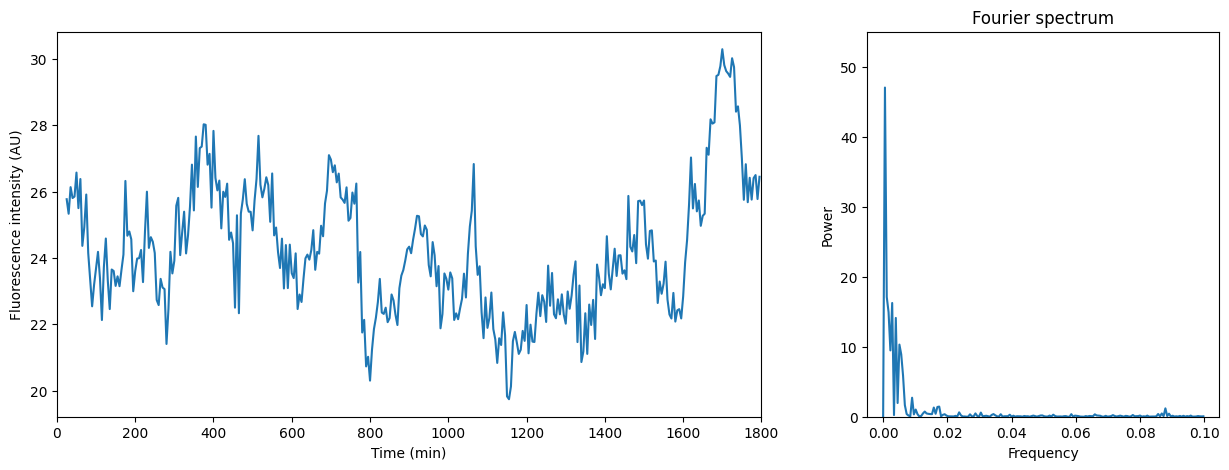
\includegraphics[width=\textwidth]{fft_raw}
   \caption{
     Raw signal
   }
   \label{fig:analysis-filter-raw}
  \end{subfigure}
  \begin{subfigure}[htpb]{0.8\textwidth}
   \centering
   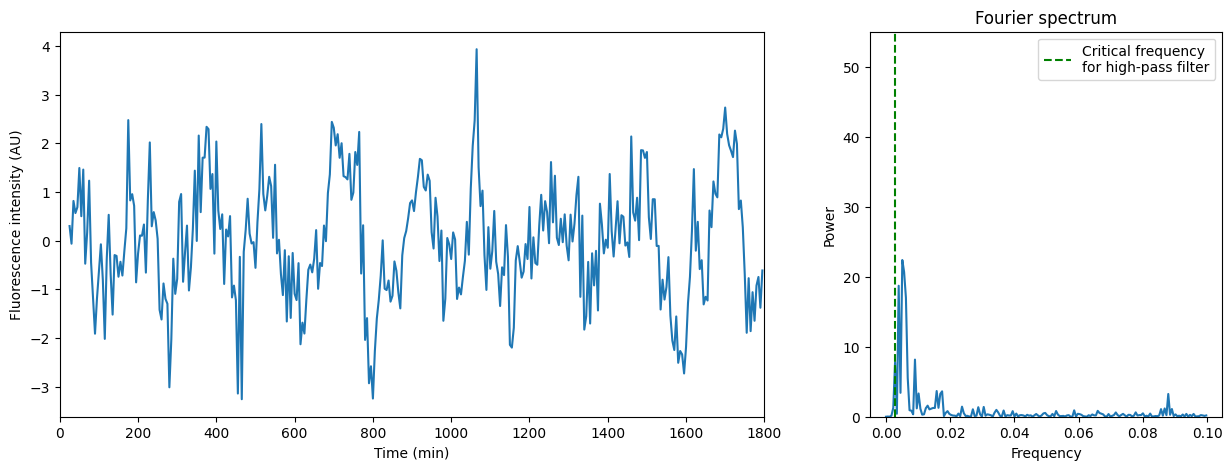
\includegraphics[width=\textwidth]{fft_butterworth}
   \caption{
     Signal processed with high-pass butterworth filter of frequency \SI[parse-numbers=false]{1/350}{\minute^{-1}}.
   }
   \label{fig:analysis-filter-butterworth}
  \end{subfigure}
  \begin{subfigure}[htpb]{0.8\textwidth}
   \centering
   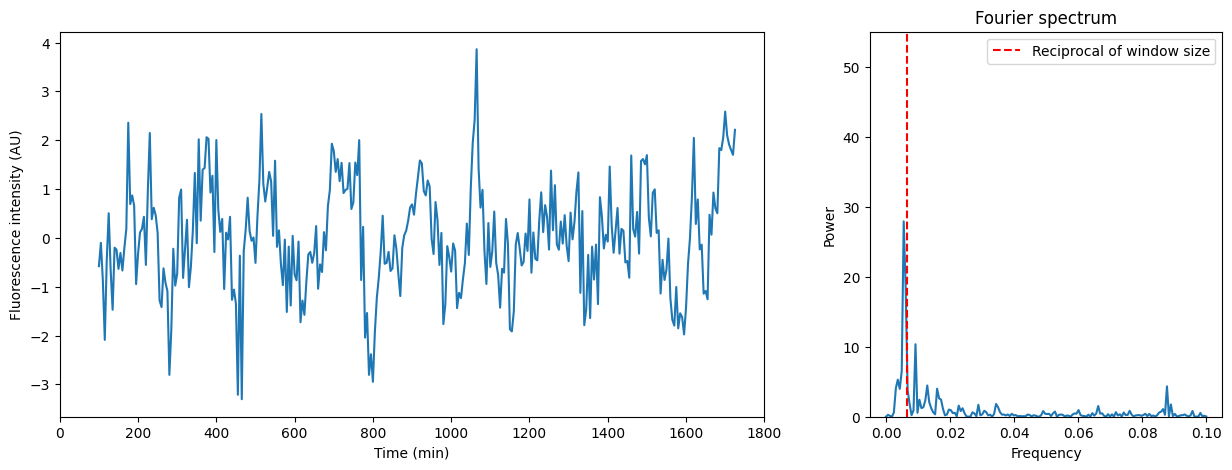
\includegraphics[width=\textwidth]{fft_slidingwindow}
   \caption{
     Signal processed by subtracting moving average with window size 30.
   }
   \label{fig:analysis-filter-slidingwindow}
  \end{subfigure}
  \begin{subfigure}[htpb]{0.8\textwidth}
   \centering
   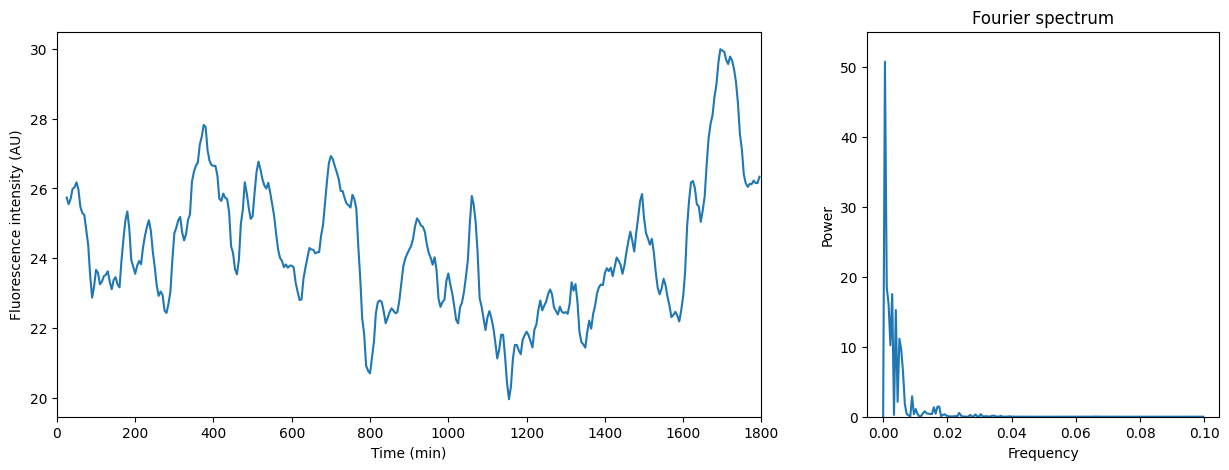
\includegraphics[width=\textwidth]{fft_savgol}
   \caption{
     Signal processed with Savitzky-Golay filter (window size 7, polynomial order 3).
   }
   \label{fig:analysis-filter-savgol}
  \end{subfigure}
  \caption[
    Different filtering methods
  ]{
    Different filtering methods result in different effects to both the signal (left panels) and the Fourier spectrum of the signal (right panels).
  }
  \label{fig:analysis-filter}
\end{figure}

For filtering time series, I have considered sliding-window methods and methods that modify the frequency profile of the time series.

Alternatively, I consider methods that modify the frequency profile of the time series.
Defining a high- or low-pass filter offers direct control over frequencies, but the user must use a judgement call to define a critical frequency.
In my case, I define the critical frequency for a high-pass Butterworth filter as \SI[parse-numbers=false]{1/350}{\minute^{-1}} as this corresponds to the upper limit of reasonable durations of yeast metabolic cycles and cell division cycles that I have observed in my single-cell microfluidics experiments (figure~\ref{fig:analysis-filter-butterworth}).
Defining a critical frequency in such a way will exclude the possibility of metabolic cycles that go on for longer; however, this is a trade-off I am willing to make so that I can extract the individual oscillations better.

Thus, for subsequent analysis, I use the high-pass Butterworth filter defined above to process raw fluorescence time series.
This is because using this method, I have more control over the frequency components, and the methods preserves noise frequencies that are useful for assessing the quality of the data set (to be discussed later in this section) and estimating the noise properties (to be discussed in section~\ref{subsec:analysis-characterisation-acf}).

However, sliding-window methods have caveats.
Subtracting a moving average relies on knowing a window size that approximates the expected oscillation period, gives no control over the signal frequencies, introduce artefacts in the frequency spectrum, and decreases the number of time points available (figure~\ref{fig:analysis-filter-slidingwindow}).
Such methods may distort the data in a way that affects conclusions.
Additionally, if the time series is processed with such methods, it is not possible to restore the raw data.


% However, there are challenges with classification of noisy biological time series with relatively few time points.
% In addition, such a classification task necessarily needs a cut-off somewhere, thus requiring judgement calls.
% You'd see this crop up in this section multiple times when I discuss my methods and I reveal different angles of approaching this.

Determining whether a time series is oscillatory, or rhythmicity detection, is technically difficult for several reasons.
From a signal processing perspective, any time-dependent signal can be decomposed into a combination of sinusoids of different frequencies.
Noise typically manifests as high-frequency components while trends manifests as low-frequency components --- the filtering methods in section~\ref{sec:analysis-cleaning} arise because of this fact.
It is thus more reasonable to detect the presence of a frequency within the range of interest.
However, this depends on knowing an expected range of frequencies.
When studying the circadian rhythm, this is often the case: studies expect rhythms of around \SI{24}{\hour} and \textcite{zielinskiStrengthsLimitationsPeriod2014} uses the range of \SIrange{16}{32}{\hour} for rhythmicity detection.
This method is less useful when the frequency of oscillations is unknown or known to be in a wide range of frequencies, as is the case for the yeast metabolic cycle.
Furthermore, there is no way to objectively specify a failure rate for a rhythmicity detection method as there is no independent method to estimate rhythmicity \parencite{zielinskiStrengthsLimitationsPeriod2014}, therefore such a classification method requires a subjective definition of whether each time series is oscillatory.
In other words, this is similar to the requirement of a training data set with human-defined labels, and thus a human-defined failure rate, for supervised machine learning.

%I then compared the classification results against manual classification of these time series into oscillating and non-oscillating.
The classifier was able to rank the time series by quality of oscillation (Fig.\ \ref{fig:ClassifierBestWorstTS}).
The peak of the normalised classical periodogram of each time series was used as a proxy for the quality of oscillation (Fig.\ \ref{fig:ClassifierBestWorstPS}).
By eye, birth events coincided with peaks of some higher-quality oscillations.
However, this was also true for some oscillations ranked as lower-quality.
% [COMMENTED -- don't think this sentence is really consequential, and the proposed plot doesn't add much] Additionally, higher-quality oscillations do not seem to be associated with imaging positions/flavin LED exposure times. % FIGURE: scatter plot, horizontal axis is rank, vertical axis is imaging position
% Wee bit of discussion (plus a plot to illustrate my point).  Deeper discussion about multiple main frequencies is in discussion, and has references to literature.

When performing a classification task, Each piece of input data has a label assigned to it to denote which category it belongs to.
The input data set is then divided into a training data set and a test data set.
The machine learning model is then fit on the training data set to fit parameters in the model, and then the performance of the model is evaluated on the test data set.
Such model evaluation is based on quantitative measures of how well the model matches data to appropriate labels.

% -----[Probably no need to go into so much detail.]-----
% I removed the first 25 time points that is most likely cells adapting to microfluidic conditions.
% I also removed time points after time point 168, when nutrient switching occurred.
% I removed all time series with missing time points.
In total, there are 294 cells, each with 118 time points, spaced 5 minutes apart.

% Figure ... shows a clear downwards trend (which I can't explain biologically yet). If an SVM model is trained using time points as features, there is a risk that the model recognises this trend rather than the presence of oscillations.
% This plot highlights the risk: for some reason non-oscillating time series (hand-scored) tends to have a smaller gradient.
% I thus detrended the data by generating a moving average with a sliding window size of 45 time points, and then dividing each data point by the moving average. I chose 45 time points because that covers ~3 cell division cycles.
% However, there are caveats.
% If the cell division cycle length differs, this window length should change; a spectral method (FFT, autoregressive) could give me an idea of what this cell division cycle length is.
% Additionally, this decreases the number of time points --- there are now 98.

I explored support vector machine (SVM) and random forest (RF) model architectures.
First, I used an support vector classifier (SVC) with these hyperparameters:
\begin{enumerate}
  \item A radial bias kernel.
  \item The kernel coefficient $\gamma = 1/N$, where $N$ is the number of features.
  \item The regularisation parameter $C = 1$.  The strength of regularisation is inversely proportional to $C$.
\end{enumerate}

And, I explored three methods of featurisation: using time points as features, the time series' Fourier spectrum as features, and using \textit{catch22} features \parencite{lubbaCatch22CAnonicalTimeseries2019}.

\textit{catch22} is based on the \textit{hctsa} toolbox \parencite{fulcherHctsaComputationalFramework2017} developed to compute vectors of features for time series.
This toolbox contains 7701 features defined from across the time series analysis literature.
I focused on the 22-feature \textit{catch22} subset of the original 7701 features (table \ref{tab:catch22}).
\textcite{lubbaCatch22CAnonicalTimeseries2019} selected these 22 features because they minimise redundancy while maintaining classification performance across 93 test datasets.
This feature set excludes features that are dependent on mean or spread.

After featurisation, to account for the different dynamic ranges of each feature, the features were scaled by computing the standard score, similar to equation~\ref{eq:analysis-stdscore}.

As a control, I randomly assigned time series to the oscillatory and non-oscillatory categories and used their time series as features.
I then evaluated the model using stratified five-fold cross-validation, using precision and recall as evaluation metrics.
Using time points as features, the metrics show that precision and recall is better than random, and stratified five-fold cross-validation does not suggest overfitting (figure~\ref{fig:analysis-precision-recall}).
Using the Fourier spectrum as features, precision and recall are comparative as with using time points as
features.
However, there seems to be greater variation in these measures.

Nevertheless, precision and recall are best with \textit{catch22}.
Feature vectors seem to suggest that the \texttt{FC\_LocalSimple\_mean3\_stderr} feature (represented as feature 9 in figure~\ref{fig:analysis-svc-catch22}) plays an important role in distinguishing the oscillatory and non-oscillatory time series.
This feature is defined as the mean error from a rolling 3-sample mean forecasting.


The importance of characterising my time series is that I can quantify how my yeast metabolic cycles respond to genetic and nutrient perturbations.
Here, I discuss characterising periods, phases, and amplitudes of the oscillations.
%Note that I discuss many of the same non-machine learning methods as I did for the classification section -- such methods are often developed for characterisation but offer features that are useful for classification, but it makes more sense in my thesis to order it this way because you'd usually try to filter out the non-oscillatory time series before trying to grab properties of the oscillatory ones.
Then I will discuss the merit of combining several methods, given the limitations of analysing noisy biological time series that I have found.
% [THIS SENTENCE MAY GO]
%Characterisation is also intimately related to classification, in particular the machine learning methods: these methods can be adapted to tell apart different strains (presumably of different shapes) rather than telling apart oscillatory and non-oscillatory time series.

% Literature review subsection
% STEAL IDEAS FROM: ZIELINSKI ET AL. 2014
\subsection{Periods, phases, amplitudes}
\label{subsec:analysis-characterisation-quantities}

Three useful characteristics of a time series include its period, its phase relative to a reference, and its amplitude.
% Adapted from meeting with Zielinski.
% TODO with this:
% - support with evidence, e.g. discussion points from his paper and others

% PERIOD
The period of an oscillatory time series is the easiest characteristic to compute a fixed number for because it is well-defined.

% SHAPE
The shape of oscillations in a time series is difficult to analyse and assign a meaningful quantitative measure to --- it is easier to describe the shape by eye.
From the signal processing point of view, the shape of an oscillation is defined by a set of frequencies of sinusoids and their respective power values.
In other words, to quantitatively describe the shape of an oscillation, a vector of values is needed, and any fixed-number representation necessarily removes some information about the shape.
Alternatively, the shape can be expressed in terms of skewness, treating one oscillation as if it were a probability distribution. %[CITATION NEEDED].

% PHASE
There are challenges in obtaining a fixed number of represent the phase of an oscillator time series based on the signal.
Most importantly, the phase must be defined with respect to a human-defined reference, which may not be clear depending on the data.
In addition, the phase angle can have uncertainty, particularly if the time series is noisy.
Phase estimation is part of period estimation methods that are based on fitting cosines to data (to be discussed later), and an error range will always be given.
Estimating the phase angle also requires multiple replicates as estimation methods rely on plotting populations of time series and seeing if they overlap.
Modular arithmetic is also needed for such methods.
In sum, more information is needed to estimate the phase compared to other methods.
When a quantitative representation of the phase is obtained, it can be expressed in absolute terms (in units of time), or in relative terms with respect of the period (in radians).

% AMPLITUDE
The amplitude of the time series is easiest to compute and easiest to explain.
Methods to estimate the amplitude relies on fitting a cosine to the signal.
Such methods are adequate if the shape of the time series does not change by much across time, but are inadequate if oscillations are skewed, as the cosine function models symmetrical oscillations.
However, the amplitude is likely the least important characteristic to study in the biological timekeeping field.

Of these, finding the period is the easiest to do and most pertinent for my investigation of the yeast metabolic cycle, so I focus my further discussion on period estimation.
Another common period-estimation method relies on the autocorrelation function, and it was used in \textcite{papagiannakisAutonomousMetabolicOscillations2017}.
Here, I am going to discuss adapting the autocorrelation function for my data.
